% Template for Elsevier CRC journal article
% version 1.2 dated 09 May 2011

% This file (c) 2009-2011 Elsevier Ltd.  Modifications may be freely made,
% provided the edited file is saved under a different name

% This file contains modifications for Procedia Structural Integrity

% Changes since version 1.1
% - added "procedia" option compliant with ecrc.sty version 1.2a
%   (makes the layout approximately the same as the Word CRC template)
% - added example for generating copyright line in abstract

%-----------------------------------------------------------------------------------

%% This template uses the elsarticle.cls document class and the extension package ecrc.sty
%% For full documentation on usage of elsarticle.cls, consult the documentation "elsdoc.pdf"
%% Further resources available at http://www.elsevier.com/latex

%-----------------------------------------------------------------------------------

%%%%%%%%%%%%%%%%%%%%%%%%%%%%%%%%%%%%%%%%%%%%%%%%%%%%%%%%%%%%%%
%%%%%%%%%%%%%%%%%%%%%%%%%%%%%%%%%%%%%%%%%%%%%%%%%%%%%%%%%%%%%%
%%                                                          %%
%% Important note on usage                                  %%
%% -----------------------                                  %%
%% This file should normally be compiled with PDFLaTeX      %%
%% Using standard LaTeX should work but may produce clashes %%
%%                                                          %%
%%%%%%%%%%%%%%%%%%%%%%%%%%%%%%%%%%%%%%%%%%%%%%%%%%%%%%%%%%%%%%
%%%%%%%%%%%%%%%%%%%%%%%%%%%%%%%%%%%%%%%%%%%%%%%%%%%%%%%%%%%%%%

%% The '3p' and 'times' class options of elsarticle are used for Elsevier CRC
%% The 'procedia' option causes ecrc to approximate to the Word template
\documentclass[3p,times,procedia]{elsarticle}
\flushbottom

%% The `ecrc' package must be called to make the CRC functionality available
\usepackage{ecrc}
%\usepackage{amsmath}

\usepackage[bookmarks=false]{hyperref}
    \hypersetup{colorlinks,
      linkcolor=blue,
      citecolor=blue,
      urlcolor=blue}
  
\usepackage{booktabs}
\usepackage{comment}

%% The ecrc package defines commands needed for running heads and logos.
%% For running heads, you can set the journal name, the volume, the starting page and the authors

%% set the volume if you know. Otherwise `00'
\volume{00}

%% set the starting page if not 1
\firstpage{1}

%% Give the name of the journal
\journalname{Structural Integrity Procedia}

%% Give the author list to appear in the running head
%% Example \runauth{C.V. Radhakrishnan et al.}
\runauth{Cochet et al.}

%% The choice of journal logo is determined by the \jid and \jnltitlelogo commands.
%% A user-supplied logo with the name <\jid>logo.pdf will be inserted if present.
%% e.g. if \jid{yspmi} the system will look for a file yspmilogo.pdf
%% Otherwise the content of \jnltitlelogo will be set between horizontal lines as a default logo

%% Give the abbreviation of the Journal.
\jid{prostr}

%% Give a short journal name for the dummy logo (if needed)
%\jnltitlelogo{Procedia Structural Integrity}

%% Hereafter the template follows `elsarticle'.
%% For more details see the existing template files elsarticle-template-harv.tex and elsarticle-template-num.tex.

%% Elsevier CRC generally uses a numbered reference style
%% For this, the conventions of elsarticle-template-num.tex should be followed (included below)
%% If using BibTeX, use the style file elsarticle-num.bst

%% End of ecrc-specific commands
%%%%%%%%%%%%%%%%%%%%%%%%%%%%%%%%%%%%%%%%%%%%%%%%%%%%%%%%%%%%%%%%%%%%%%%%%%

%% The amssymb package provides various useful mathematical symbols

\usepackage{amssymb,amsmath,amsthm,enumitem}
\usepackage{siunitx}
\usepackage{physics}
\usepackage{float}
\usepackage{xpatch}
\usepackage{mathtools, nccmath}
\xpatchcmd{\NCC@ignorepar}{%
\abovedisplayskip\abovedisplayshortskip}
{%
\abovedisplayskip\abovedisplayshortskip%
\belowdisplayskip\belowdisplayshortskip}
{}{}

%% The amsthm package provides extended theorem environments
%% \usepackage{amsthm}

%% The lineno packages adds line numbers. Start line numbering with
%% \begin{linenumbers}, end it with \end{linenumbers}. Or switch it on
%% for the whole article with \linenumbers after \end{frontmatter}.
%% \usepackage{lineno}

%% natbib.sty is loaded by default. However, natbib options can be
%% provided with \biboptions{...} command. Following options are
%% valid:

%%   round  -  round parentheses are used (default)
%%   square -  square brackets are used   [option]
%%   curly  -  curly braces are used      {option}
%%   angle  -  angle brackets are used    <option>
%%   semicolon  -  multiple citations separated by semi-colon
%%   colon  - same as semicolon, an earlier confusion
%%   comma  -  separated by comma
%%   numbers-  selects numerical citations
%%   super  -  numerical citations as superscripts
%%   sort   -  sorts multiple citations according to order in ref. list
%%   sort&compress   -  like sort, but also compresses numerical citations
%%   compress - compresses without sorting
%%
\biboptions{authoryear}

% \biboptions{}

% if you have landscape tables
\usepackage[figuresright]{rotating}
\usepackage{graphicx}
\usepackage{subcaption}
%\usepackage{harvard}
% put your own definitions here:x
%   \newcommand{\cZ}{\cal{Z}}
%   \newtheorem{def}{Definition}[section]
%   ...

% add words to TeX's hyphenation exception list
%\hyphenation{author another created financial paper re-commend-ed Post-Script}

% declarations for front matter

\begin{document}
\begin{frontmatter}

%% Title, authors and addresses

%% use the tnoteref command within \title for footnotes;
%% use the tnotetext command for the associated footnote;
%% use the fnref command within \author or \address for footnotes;
%% use the fntext command for the associated footnote;
%% use the corref command within \author for corresponding author footnotes;
%% use the cortext command for the associated footnote;
%% use the ead command for the email address,
%% and the form \ead[url] for the home page:
%%
%% \title{Title\tnoteref{label1}}
%% \tnotetext[label1]{}
%% \author{Name\corref{cor1}\fnref{label2}}
%% \ead{email address}
%% \ead[url]{home page}
%% \fntext[label2]{}
%% \cortext[cor1]{}
%% \address{Address\fnref{label3}}
%% \fntext[label3]{}

\dochead{ICSI 2023 The 5th International Conference on Structural Integrity}%

\title{Direct Assessment of Mode I Fracture Properties in Silver Fir Using MMCG Specimen and Digital Image Correlation}

%% use optional labels to link authors explicitly to addresses:
%% \author[label1,label2]{<author name>}
%% \address[label1]{<address>}
%% \address[label2]{<address>}

\author[a]{O. Cochet}
\author[b,c]{J. Xavier\corref{cor1}}
\author[b,c]{R.F. Martins}
\author[a]{R. Moutou Pitti}


\address[a]{Université Clermont Auvergne, Clermont Auvergne INP, Institut Pascal, Clermont-Ferrand, France}
\address[b]{UNIDEMI, Department of Mechanical and Industrial Engineering, NOVA School of Science and Technology, Universidade NOVA de Lisboa, 2829-516 Caparica, Portugal}
\address[c]{Laboratório Associado de Sistemas Inteligentes, LASI, 4800-058 Guimarães, Portugal}


\begin{abstract}
In this study, we investigate the cracking behaviour of softwood species using MMCG specimens. We aim to accurately determine crack length during fracture propagation and related fracture parameters, which is often challenging to obtain in wood. To achieve this, we employ the Arcan system to load the specimen, which has the advantage of inspecting from pure to mixed mode fracture loading to activate different failure modes. Digital Image Correlation (DIC) measures displacement and strain fields near the crack.
Our primary focus is on open I mode crack growth, and we generate force versus crack opening curves from the measurements. In addition, we use the imposed displacement compliance method to determine the strain energy release rate for opening mode.
This study highlights the importance of fracture mechanics in ensuring the safety and reliability of wooden structures. Knowledge of the fracture parameters of wood can aid in the design and development of more efficient and sustainable wooden products. Accurate determination of crack length is critical in this regard. Therefore, using digital image correlation techniques and imposed displacement compliance methods can improve our understanding of the fracture behaviour of wood and aid in the design of more reliable and efficient wooden structures.
\end{abstract}

\begin{keyword}
Digital image correlation \sep Mode I \sep Fracture parameters \sep Wood
\end{keyword}
\cortext[cor1]{Corresponding author. Tel.: +351 212 948 567.}
\end{frontmatter}
%\correspondingauthor[*]{Corresponding author. Tel.: +0-000-000-0000 ; fax: +0-000-000-0000.}
\email{jmc.xavier@fct.unl.pt}

% \begin{nomenclature}
% \begin{deflist}[A]
% \defitem{A}\defterm{radius of}
% \defitem{B}\defterm{position of}
% \defitem{C}\defterm{further nomenclature continues down the page inside the text box}
% \end{deflist}
% \end{nomenclature}

\begin{comment}
\begin{nomenclature}
	\begin{deflist}[A]
		\defitem{CIRAD}\defterm{\textbf{C}entre (de coopération) \textbf{I}nternnationale (en) \textbf{R}echerche}
		\defitem{CTOD}\defterm{\textbf{C}rack \textbf{T}ip \textbf{O}pening \textbf{D}isplacement}
		\defitem{CTS}\defterm{\textbf{C}rack \textbf{T}ip \textbf{O}pening \textbf{D}isplacement}
		\defitem{DCB}\defterm{\textbf{D}ouble \textbf{C}antilever \textbf{B}eam}
		\defitem{DIC}\defterm{\textbf{D}igital \textbf{I}mage \textbf{C}orrelation}
		\defitem{CTS}\defterm{\textbf{C}rack \textbf{T}ip \textbf{O}pening \textbf{D}isplacement}
		\defitem{MMCG}\defterm{\textbf{M}ixed \textbf{M}ode \textbf{C}rack \textbf{G}rowth}
		\defitem{WS}\defterm{\textbf{W}edge \textbf{S}plitting}
		\defitem{CTS}\defterm{\textbf{C}rack \textbf{T}ip \textbf{O}pening \textbf{D}isplacement}
	\end{deflist}
\end{nomenclature}
\end{comment}

%\enlargethispage{-7mm}
\section{Introduction}\label{S:intro}

Wood is a natural, renewable, low energy cost, recyclable and biologically degradable material. Wood is an increasingly popular engineering material due to its potential for reducing pollution and combating global warming. Its use in structural applications has been recognised as a promising solution for sustainable and efficient building design. However, ensuring the safety and reliability of wooden structures requires a comprehensive understanding of the fracture mechanics of wood. Studying the failure properties of wood is therefore crucial to further enhance adding-value structural applications.

The present document aims to study mechanical fracture of wood in mode I on Silver Fir specimens of type MMCG. The proposed work consists mainly in conducting measurements carried out by kinematic field measurements obtained by the method known as image correlation or DIC. Integrating the DIC method through the MatchID software and subsequent Python-based data processing will be instrumental in attaining the desired outcomes. Two Python programs will be compared in order to verify the acuity of each method. This project consists of modelling the observed behaviour, both from the crack initiation and propagation point of view. The study will focus solely on a single wood species, and variations in wood moisture content will not be considered. The tests were carried out in a universal testing machine with a homemade Arcan fixture. This data can be used in future studies to develop computational simulations of fracture testing to determine fracture parameters from inverse methods.

%\cite{Dong201975}
\section{Methods}\label{S:method}

\subsection{Material and MMCG fracture test}\label{Ss:spec}

The MMCG fracture test was initially developed by \citet{MoutouPitti2008}. The proposed fracture test is a compromise between DCB and CTS fracture tests, to obtain different mixing rates under a stable crack propagation. The nominal geometry of the MMCG specimen is shown in Figure~\ref{F:Fig1}a.

% \begin{figure}[th]
% 	\centering
% 	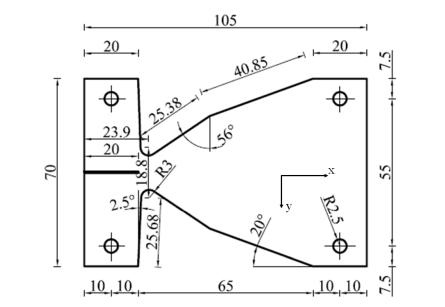
\includegraphics[width=0.4\textwidth]{Figures/fig23}
% 	\caption[MMCG specimen]{dimensions and geometry of Mixed Mode Crack Growth specimen}
% 	\label{fig:Fig5}
% \end{figure}

Fracture test were carried out on Silver Fir, which belongs to the category of coniferous trees. This softwood species is predominantly found in the northern hemisphere, similar to pines and other aged trees. Its name originates from the white colour of its wood, and its circumference typically ranges from 50 to 80 cm. According to CIRAD data, the Silver Fir exhibits a density of 0.45 to 0.60, a saturation fiber point (SFP) of approximately 30\%, and a compressive strength of 41 MPa \citep{Angellier2017}. Wooden specimens were carefully characterised before testing by measuring weight, density, and moisture content. Before the tests, the samples were weighed, denoted as $M_H$, to determine their mass during testing. The wood density can also be derived from the sample's volume and mass. The density of each sample can be determined by applying the formula $\rho = M/V$.
After testing, the specimens were placed in an oven set at 100 degrees until their mass, labelled as $M_C$, stabilised. Two specimens were subjected to this process for 73 hours, and various measurements were taken until a constant mass was achieved. The moisture content of the specimens were then determined: $(M_{H}-M_{0})/M_{0}$ (\%). In summary, specimens had an average mass $M_H$ of 29.83g, a density of 431.3kg/m$^3$, and a moisture content of 10.3\%.

An Arcan fixture system is required to perform the MMCG fracture tests. Indeed, this part allows the connection of the MMCG wood specimen to the cross-head displacement of the test frame. Figure~\ref{F:Fig1}b shows the Arcan device we will use, inspired by the thesis of \citep{Odounga2018phd}. The fixing holes enables to load the specimen with different angular values of the angle in relation to the vertical direction in order to activate different failure modes depending on the load angle.  The fixture was designed and assembled using SolidWorks software, and detailed technical drawings were produced for manufacturing (Figure~\ref{F:Fig1}b).

The fracture tests were performed using a MTS Servohydraulic testing machine with a maximum capacity of 100 kN. Figure~\ref{F:Fig1}c shows the experimental set-up, which includes the Arcan fixture and the optical camera-lens-illumination devices. The Arcan fixture was mounted to the testing machine using standard bolts, with washers inserted between the specimen and the Arcan system to reinforce the attachment points. To facilitate specimen changes between tests, manual controls were employed to elevate the moving part of the testing machine, minimising residual tension between the bolt holes and the Arcan system. Furthermore, before testing, an arbitrary pre-load was applied to the specimen to prevent any clearance or unintended movement of the specimen (which could cause image defocusing). Load and cross-head displacement data were recorded at a frequency of 5 Hz. Additionally, a real-time plot was generated during the test for visualisation.

% \begin{figure}[htp]
% 	\begin{minipage}[c]{.46\linewidth}
% 		\centering
% 		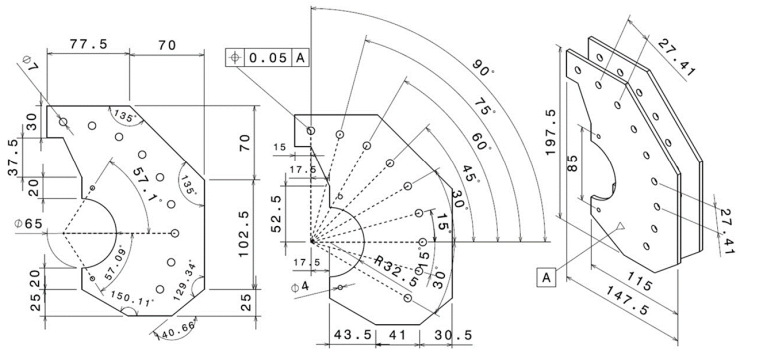
\includegraphics[scale=0.4]{Figures/fig24}
% 		\caption{Size of the Arcan fastening system \citep{Odounga2018phd}.}
% 		\label{fig:Fig6}
% 	\end{minipage}
% 	\hfill%
% 	\begin{minipage}[c]{.46\linewidth}
% 		\centering
% 		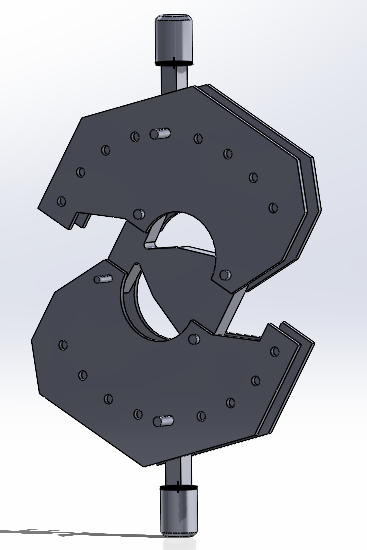
\includegraphics[scale=0.4]{Figures/fig26}
% 		\caption{Assembled device in Solidworks.}
% 		\label{fig:Fig8}
% 	\end{minipage}
% \end{figure}

\subsection{Optical set-up and settings}\label{Ss:optical}

The optial system used an Alvium 1800 U-2040m Allied Vision camera and a 60 mm Nikkor lens for image grabbing and acquisition. The camera has a resolution of 4512 (H) $\times$ 4512 (V) and a sensor size of type 1.1. The front of the lens was positioned at a working distance of 285 mm with an aperture of f/11 and an exposure time of 60 milliseconds. The cross-head displacement of the testing machine was 0.02mm/s, and the camera had a frequency of 1 Hz (1 fps).
A green illumination set-up was used to enhance the sensitivity of the sensor. Notably, care was taken during lens and camera adjustments to optimise focusing and exposure time, ensuring an appropriate spread of light intensity to prevent pixel saturation in the sensor. The camera was securely mounted on a tripod to ensure a stable position relative to the specimen's target surface, enabling the capture of consistent images throughout the tests. The frontal face of the specimens was coated with a suitable speckle pattern. A first layer of white paint was added and a cloud of black dots formed a second layer of paint to create a distinctive local pattern across the region of interest (ZOI) ahead of the crack tip. Additionally, a scale positioned in the surface plane was employed to establish the conversion factor for translating pixels into millimetres.

% \begin{figure}[htbp]
% 	\centering
% 	\begin{tabular}{cc}
% 		\begin{minipage}{0.3\textwidth}
% 			\centering
% 			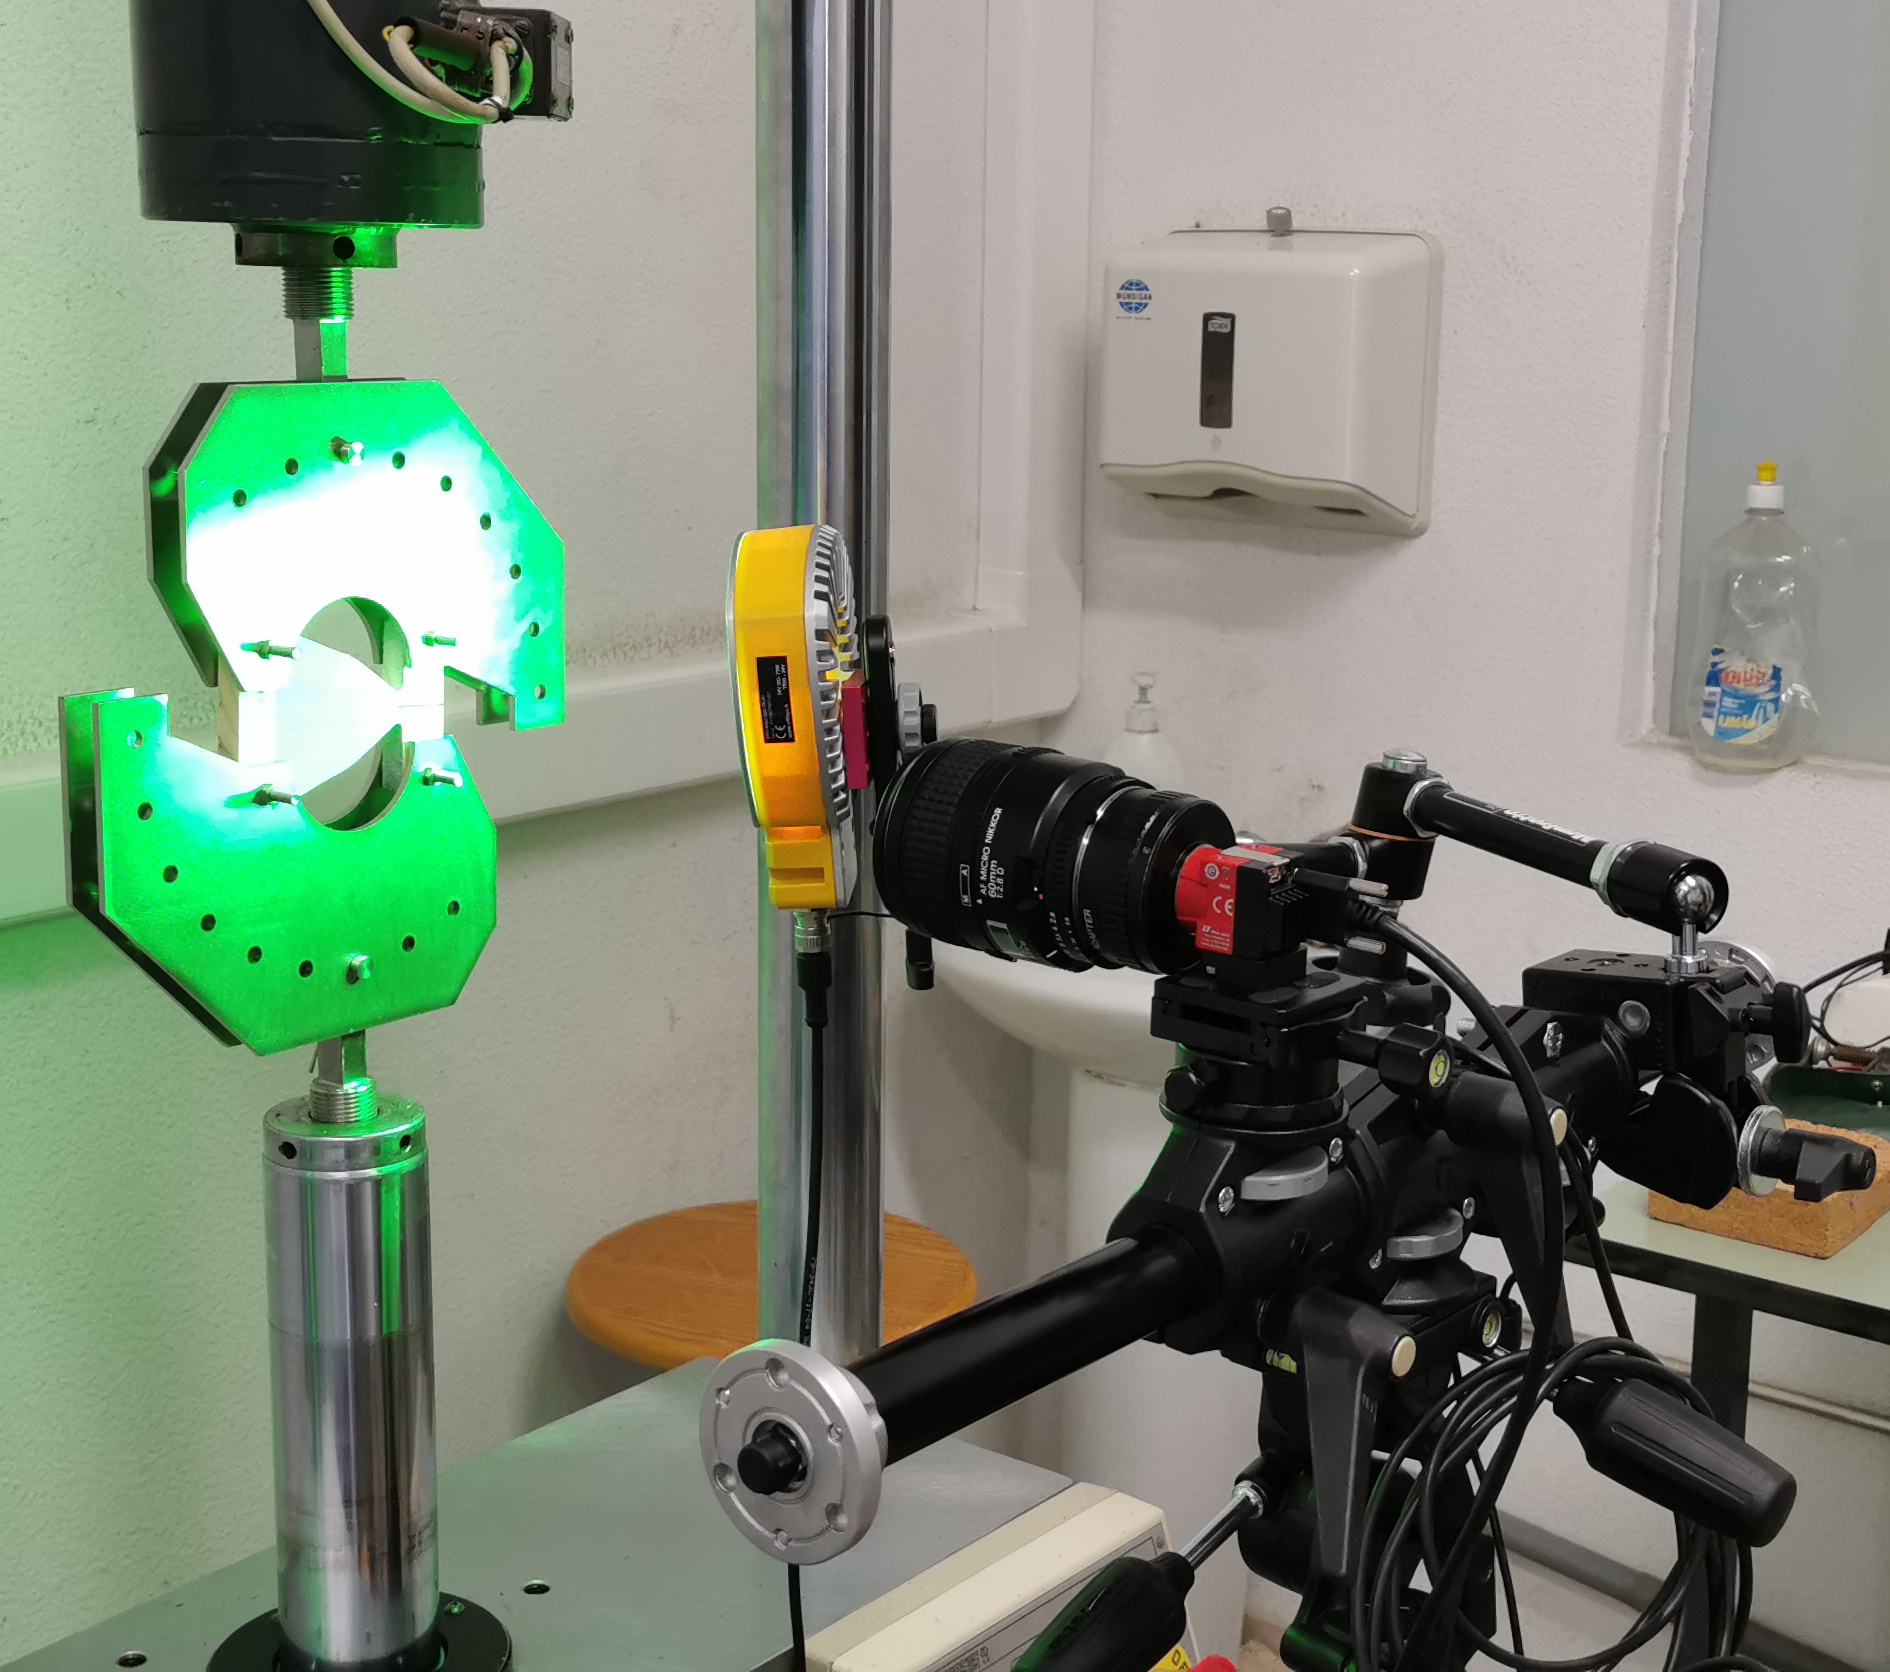
\includegraphics[width=\textwidth]{Figures/Setup0_crop}
% 			\caption{Experimental set-up.}
% 			\label{fig:Setup0°}
% 		\end{minipage} &
% 		\begin{minipage}{0.3\textwidth}
% 			\centering
% 			\includegraphics[width=\textwidth]{Figures/Speckle_DIC}
% 			\caption{Speckle pattern typically obtained with DIC Histogram of the speckle image.}
% 			\label{fig:Speckle_DIC}
% 		\end{minipage}
% 	\end{tabular}
% \end{figure}

\begin{figure}[t]
	\centering
	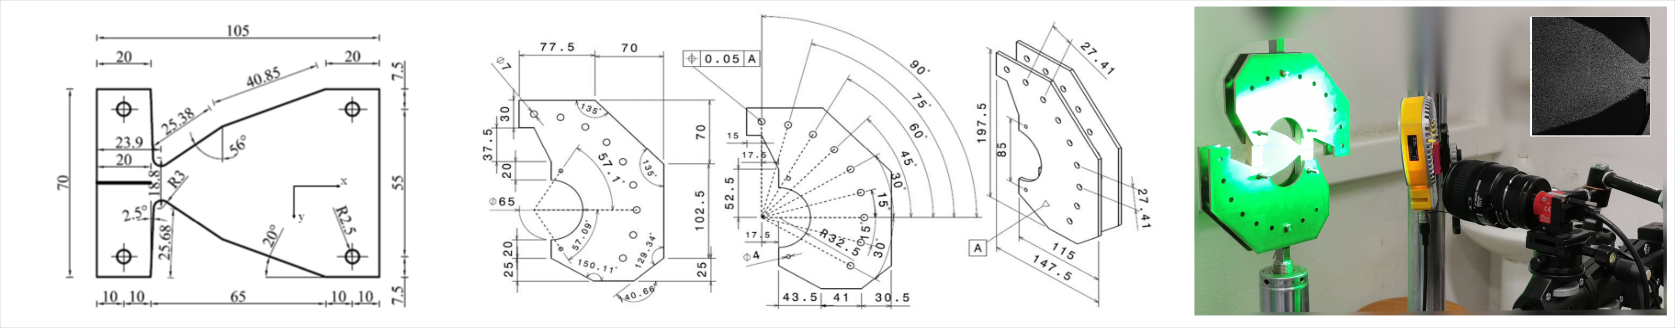
\includegraphics[width=\textwidth]{Fig1}
	\begin{minipage}{1.\textwidth}
	{\footnotesize (a) \hspace{4cm} (b) \hspace{6.5cm} (c)}
	\end{minipage}
	\caption{Experimental set-up.}
	\label{F:Fig1}
\end{figure}

\subsection{Digital image correlation}\label{Ss:dic}

In this work the MatchID DIC 2D software was used, and Python-based scripting was coded for post-processing purposes in view of the fracture parameter measurements. The focus of this study was the evaluation of crack opening displacement and crack length variation during the fracture tests with regard to the applied load. In DIC processing it is fundamental to property select the DIC settings, including subset size, subset step, strain gauge window, shape functions, and correlation criterion \citep{DICguide2018}. These parameters play a crucial role in determining the accuracy and spatial resolution of the measured displacements and reconstructed strain fields \citep{Xavier2012207,PereiraandXavier2018}. To achieve a trade-off between spatial resolution and accuracy, a parametric analysis was conducted utilizing the Parametric Module of MatchID. The resulting DIC settings are summarized in Table~\ref{tab:MatchID_param}. Subsequently, data from each analysis were extracted in a matrix format for each acquisition step. These data were then subjected to further analysis using Python scripting, with the aim of evaluating fracture parameters within the scope of this study.

\begin{table}[h]
	\centering
	\begin{tabular}{m{0.3\textwidth} m{0.4\textwidth}}
		\toprule
		\textbf{Setting} & \textbf{Selection} \\
		\midrule
		Correlation Coefficient & ZNCC \\
		Interpolation order & Bicubic Splines \\ 
		Transformation order & Quadratic \\
		Prefiltering & Gaussian \\
		Progress history & Spatial \\
		Subset size & 31 \\
		Step size & 10 \\
		Strain window size & 5 \\ 
		Virtual Strain Gauge & 71 pixels \\
		Strain interpolation & Bilinear (Q4) Lagrange polynomials \\
		Strain Convention & Green-Lagrange \\\bottomrule
	\end{tabular}
	\caption{DIC setting parameters used in the MatchID software for the analyses.}
	\label{tab:MatchID_param}
\end{table}

\subsection{DIC post-processing}

\subsubsection{Method 1: Crack propagation based on full-field displacement fields provided by DIC}

The Crack Tip Opening Displacement (CTOD) is calculated by analysing subsets positioned just above and below the subset that initially defines the crack tip position ($a_0$) in the pre-crack propagation images. The $a_0$ subset corresponds to a specific entry in row $m$ and column $n$ in matrix representation. Observing the subsets from top to bottom makes it possible to track the displacement of the crack tip and measure it accurately. The objective is to identify the most suitable pair of subsets sufficiently close to the crack for meaningful measurements without being too close or too far. Proximity to the crack ensures relevant information, while excessive proximity or distance may compromise the accuracy of measurements. Through the analysis of these displacements, the crack opening values at each step can be obtained.

% (see Figure~\ref{fig:fig29bis})

% \begin{figure}[htp]
% 	\begin{minipage}[c]{.46\linewidth}
% 		\centering
% 		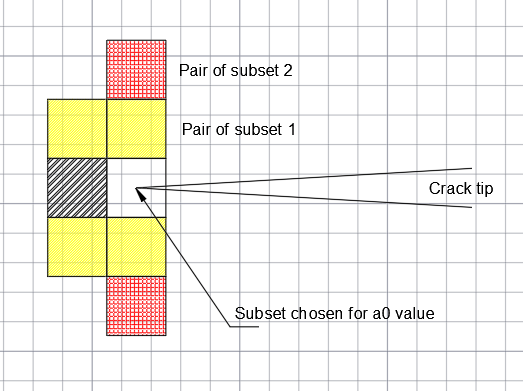
\includegraphics[scale=0.4]{Figures/fig29bis}
% 		\caption{Pair of subsets around the chosen subset $a_0$.}
% 		\label{fig:fig29bis}
% 	\end{minipage}
% 	\hfill%
% 	\begin{minipage}[c]{.46\linewidth}
% 		\centering
% 		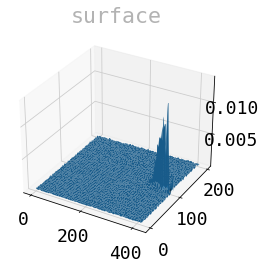
\includegraphics[scale=0.5]{Figures/A_function}
% 		\caption{A function}
% 		\label{fig:A_function}
% 	\end{minipage}
% \end{figure}

The crack length evaluation is based on the variation of the relative position between adjacent subsets, which gives an estimate of the damage occurrence. To begin with, a matching function A(x,y) is determined based on the norm of the relative position vectors as follows \citep{Xavieretal2014}:

\vspace{0pt}
\begin{equation}
	A(x,y)=\max(\lVert u_i-u_k\rVert;\lVert u_j-u_l\rVert)
	\label{eq:eq21}
\end{equation}

\noindent where $u_{i,j,k,l}$ represent the displacement vector of four adjacent subsets. A mapping mask is then defined, assuming threshold segmentation according to the following inequalities: $M(x,y) = 1, \text{ if } A(x, y) \geq \alpha \overline{A}$; $M(x,y) = 0, \text{ if } A(x, y) < \alpha \overline{A}$; $M(x,y) = -1, \text{ if } A(x, y) = \text{NaN}$. The $M$ matrix estimates the current horizontal location or crack length at a given stage. Zero values in the matrix indicate crack-free areas, while subsets within the crack or regions with missing information are given values of 1 and -1, respectively. Subsets around the crack, which are of particular interest for the study, are assigned a value of 1. By creating a sub-matrix containing -1, 0, and 1, one can visualize the damage assessment as a map, providing an overview of how the crack progresses. Tracking the furthest subset with a value of 1 helps determine the last subset where the crack tip is located. The parameter $\alpha$ acts as a cutoff tool, enabling the localization of the crack's position in the matrix's coordinate space.

% \begin{equation}
% 	M(x,y)=
% 	\begin{cases}
% 		1, & \text{if } A(x, y) \geq \alpha \overline{A} \\
% 		0, & \text{if } A(x, y) < \alpha \overline{A} \\
% 		-1, & \text{if } A(x, y) = \textrm{NaN}
% 	\end{cases}
% 	\label{eq:eq22}
% \end{equation}

% % \begin{equation}
% %     \begin{aligned}
% %     M(x,y) = 1, & \text{ if } A(x, y) \geq \alpha \overline{A}, \\
% %     M(x,y) = 0, & \text{ if } A(x, y) < \alpha \overline{A}, \\
% %     M(x,y) = -1, & \text{ if } A(x, y) = \text{NaN}.
% %     \end{aligned}
% %     \label{eq:eq22}
% % \end{equation}

The selection of the $\alpha$ parameter is not straightforward in the initial approach. To approximate its value, we first seek a correlation factor using the least squares regression method. During the test, the load-displacement curve consists of three main regions: a linear region representing a stationary zone, a second region corresponding to fracture propagation, and a third region indicating specimen rupture. By determining the correlation factor, we can identify the stage between the stationary zone and the Fracture Process Zone (FPZ). A second verification criterion based on displacement field processing is then applied to confirm the correct stage of the FPZ. By following these two steps, we can determine the stage at which the FPZ begins and the possible range of values for $\alpha$. Subsequently, we can plot the stages of crack propagation for different $\alpha$ values and assess the value of $\alpha$ that yields the largest $a(t)$ (crack length). Typically, the smallest $\alpha$ is chosen, unless a curve with simpler geometry is desired and the length of $a(t)$ remains relatively unchanged. A portion of the code enables graphical verification of the crack length by directly selecting $a_0$ and $a_f$ (final crack length). This allows the elimination of certain $\alpha$ values that do not yield the correct crack length.

\subsubsection{Method 2: Crack propagation based on crack opening displacement provided by DIC}

Method 2 uses the crack opening along the entire length of the wooden specimen to determine the length of the crack \citep{FilhoJ2022}. From the reference and current positions of the DIC calculation points, the Euclidean distance between each pair of points can be measured and the COD can be determined as:

\begin{equation}
	VD(k,i_n)=\sqrt{(x_{11bk}-x_{11tk})^2 + (x_{22bk}-x_{22tk})^2}_{i_n} - VD(k,i_0)
	\label{eq:eq23}
\end{equation}

\noindent where the indices $t$ and $b$ refer to the DIC data points located at the top and bottom of the crack path, $k$ is the index of the DIC point, $i_n$ is the image captured at time $n$, $VD(k, i_0)$ is the initial Euclidean distance between the computational points of the top and bottom reference DIC subset obtained from image $i_0$, and $x_{11}$ and $x_{22}$ are their coordinates in the image plane. VD can be defined as a displacement gauge along the crack path.

% (Figure~\ref{fig:fig30})

% \begin{figure}[htp]
% 	\centering
% 	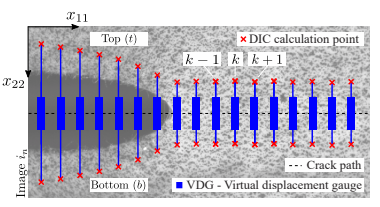
\includegraphics[width=8cm]{Figures/fig30}
% 	\caption{DIC-based virtual displacement gauge (VDG) \citep{FilhoJ2022}.}
% 	\label{fig:fig30}
% \end{figure}

\noindent The first step towards detecting the crack tip is to take the average value of $VD$ for each stage:

\begin{equation}
	\overline{VD}(i_n)=\frac{1}{k} \sum_{k=1}^{k}VD(k,i_n)
	\label{eq:eq24}
\end{equation}

\noindent The threshold value must be adjusted using the two parameters $\alpha$ and $\beta$ which are obtained by solving the equation:

\begin{equation}
		VD_{th}(i_1)=\overline{VD}(i_1)(\alpha i_1 +\beta)
		\quad\wedge\quad
		VD_{th}(i_f)=\overline{VD}(i_f)(\alpha i_f +\beta)
	\label{eq:eq25}
\end{equation}

\noindent In order to obtain $VD_{th}(i_1)$ and $VD_{th}(i_f)$, it was first necessary to read graphically the position of the crack tip of the first and last image of the Fracture Process Zone and then to find the intersection between the position of the crack tip and the crack opening VD for those two stages. Therefore, the adjusted threshold line-cut $VD_{th}(i_n)$ is given by:

\begin{equation}
	VD_{th}(i_n)=\overline{VD}(i_n)(\alpha i_n +\beta)
	\label{eq:eq26}
\end{equation}

The intersection between each $VD_{th}(i_n)$ and the corresponding $VD(k, i_n)$ curve at time n represents the $x_{11}$ position of the crack tip, denoted by ($p_n$).
It is therefore possible to calculate the growth of the crack at instant $n$:

\begin{equation}
	da_n=p_n-p_0
	\label{eq:eq27}
\end{equation}

\subsubsection{Energy release rate}

After using one of the two previous methods, we can calculate the energy release rate in mode I. To determine the Energy release rate, compliance method was chosen:

\begin{equation}
	G_\text{I}=\displaystyle\frac{{F_{c}}^2}{2b}\ \frac{\partial C}{\partial a} \quad \text{with} \quad C=\frac{v}{F_{c}} 	
	\label{eq:Energy release rate equation}
\end{equation} 
 
\noindent where: $G_c$ is the value of energy release rate (in \si{\joule\per\square\meter}); $F_c$ is the critical force which involves the crack (in \si{\newton}); $b$ is the thickness of the specimen (in \si{\milli\meter}); $v$ is the crack opening displacement according to $y$.


\section{Results and Discussion}\label{S:res}


In the Figure \ref{fig:images}, a characteristic load-displacement curve can be seen. Normally four distinct parts are observed on a load-displacement curve for Mode I fracture loading:

\begin{itemize}
	\item A small area visible at the beginning of the curve which corresponds to the setting up of the loaded specimen. 
	\item A nearly linear region arises from the elastic loading phase with a static crack front.
	\item The third segment is distinguished by a series of critical force peaks, which signify a distinct crack initiation. The progressive increase in these peaks confirms the crack's stability zone.
	\item Lastly, the final segment entails the material's rupture, which transpires when an ultimate force is applied, marking the instability of the crack.
\end{itemize}

It is followed by a plot of the crack lengths estimated by methods 1 and 2. The blue dots are crack lengths estimated graphically using MatchID and strain fields to check that the crack length estimated by Python is correct. Finally, the two other plots represent G with method 1 and 2 and show that G reaches a sort of plateau, corresponding to a stabilised propagation range.

\begin{figure}[t]
	\centering
	\begin{subfigure}[b]{0.475\textwidth}
		\centering
		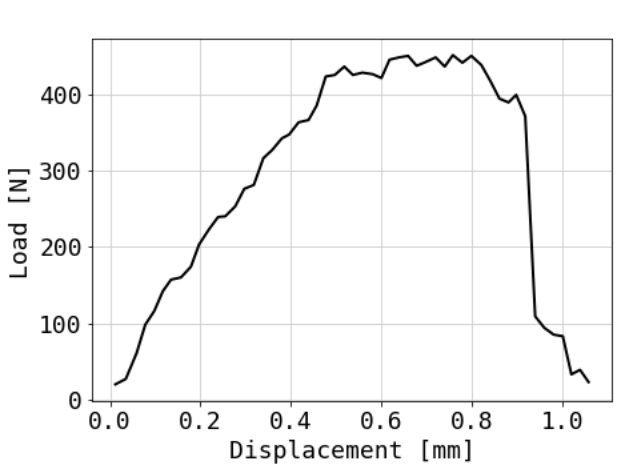
\includegraphics[width=.9\textwidth]{Fig2a}
		\caption{}
		\label{fig:image1}
	\end{subfigure}
	\hfill
	\begin{subfigure}[b]{0.475\textwidth}
		\centering
		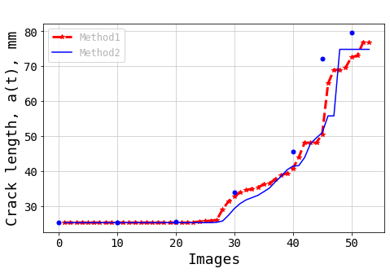
\includegraphics[width=.95\textwidth]{Fig2b}
		\caption{}
		\label{fig:image2}
	\end{subfigure}
	\\
	\begin{subfigure}[b]{0.475\textwidth}
		\centering
		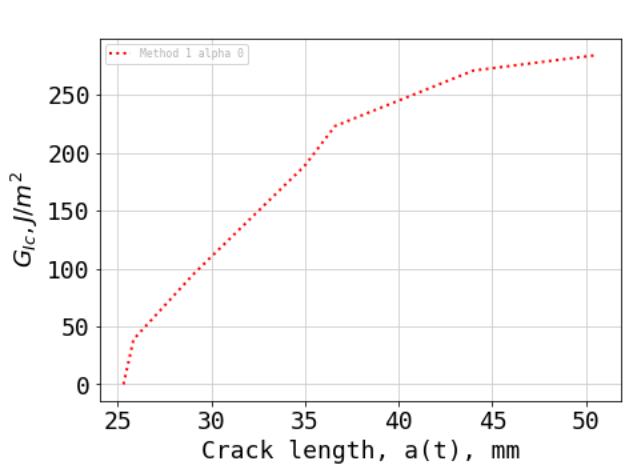
\includegraphics[width=.9\textwidth]{Fig2c}
		\caption{}
		\label{fig:image3}
	\end{subfigure}
	\hfill
	\begin{subfigure}[b]{0.475\textwidth}
		\centering
		
\includegraphics[width=.9\textwidth]{Fig2d}
		\caption{}
		\label{fig:image4}
	\end{subfigure}
	\caption{Mechanical fracture characteristics of a specimen: (a) P-Delta curve; (b) Crack length depending on time; (c) Energy release rate depending on the crack length propagation method 1; (d) Energy release rate depending on the crack length propagation method 2.}
	\label{fig:images}
\end{figure}

Table \ref{fig:fig37} compares the maximum energy release rate values obtained in this study with those reported in the literature. The comparison focuses on temperate species with similar density, moisture content ranging between 9$\%$ and 12$\%$, and an initial crack oriented in the radial-longitudinal (RL) direction. Silver Fir's average maximum energy release rate is highlighted in bold and compared to different species and test methods, including MMCG, DCB, and Wedge Splitting tests.
Firstly, it is noteworthy that the magnitude of $G$ for Silver Fir is within the same order of magnitude as other species. Silver Fir exhibits a difference of 29$\%$ compared to alder, 36$\%$ compared to Pinus pinaster, and 33$\%$ compared to Padouk. Moreover, similar values have been reported in the work of \citep{Odounga2018phd}, albeit with a standard deviation 2 to 3 times greater, indicating more dispersed results. In the study by \citep{Xavieretal2014}, experimental values of $G=190$ J/m² were also obtained, which aligns with the results of this study. Additionally, alder and Pinus pinaster exhibit similar densities (around 0.1) in comparison to Silver Fir.
The observed scattering of results can be attributed to the inherent material properties of wood, which is known for its high natural variability and anatomical composition. Furthermore, different energy release rate measurement methods and experimental parameter variations inevitably impact the final results. It is worth mentioning that the specimens in this study were predominantly derived from the extremity of the tree trunk rather than the central portion. The inclination of tree rings is apparent when observing our specimens, which could explain the slightly lower value obtained in our tests since $G_{RL} > G_{TL}$, as demonstrated in the article by \citep{Reiterer2002}.


\begin{table}
	\centering
	\resizebox{\textwidth}{!}{
		\begin{tabular}{cccccccc}
			\toprule % ligne horizontale en haut du tableau
			& References & Wood species & Test type & Orientation & Density & $G_{\max}(J/m^2)$ & Standard deviation \\
			\midrule
			& & \textbf{Silver Fir} & \textbf{MMCG} & \textbf{RL} & \textbf{0.43} & \textbf{170} & \textbf{77} \\
			& \citep{Angellier2017} & Douglas fir & DCB & RL & 0.54 & 784 &  \\
			& \cite{Angellier2017} & White fir & DCB & RL & 0.49 & 570 &  \\
			& \citep{Xavieretal2014} & Pinus Pinaster & DCB & RL & 0.543 & 270 & 64 \\
			& \citep{Reiterer2002} & Spruce & WS & RL & 0.479 & 337 & 47 \\
			& \cite{Reiterer2002} & Alder & WS & RL & 0.510 & 244 & 41 \\
			& \cite{Reiterer2002} & Oak & WS & RL & 0.553 & 348 & 38 \\
			& \citep{Reiterer2002} & Ash & WS & RL & 0.701 & 551 & 38 \\
			& \citep{Odounga2018phd} & Okoumé & MMCG & RL & 0.39-0.5 & 317 & 160 \\
			& \citep{Odounga2018phd} & Iroko & MMCG & RL & 0.56-0.7 & 323 & 200 \\
			& \citep{Odounga2018phd} & Padouk & MMCG & RL & 0.7-0.88 & 255 & 200 \\
			\bottomrule % ligne horizontale en bas du tableau
		\end{tabular}
	}
	\caption{Comparison of mean max G values for specimens in the literature, MMCG: Mixed Mode Crack Growth, DCB: Double Cantilever Beam, WS: Wedge Splitting test, RL: Radial Longitudinal.}
	\label{fig:fig37}
\end{table}

%\\\\\\\\\\\\\\\\\\\\\\\\\\\\\\\\\\\\\\\\\\\\\\\\\\\\\\\\\\

%New chapter

%\\\\\\\\\\\\\\\\\\\\\\\\\\\\\\\\\\\\\\\\\\\\\\\\\\\\\\\\\\

\section{Conclusions}\label{S:con}

This study aimed to investigate mode I fracture parameters of Silver Fir based on the MMCG specimen. An in-house Arcan fixture was used to transfer mode I loading on wooden specimens oriented in the RL propagation planes. Digital image correlation (DIC) was used to analyse the deformation and to extract crack length and crack tip opening displacement. The critical energy release rate was then directly evaluated using the compliance method. A discussion on the average $G_{max}$ values with those reported in the literature for other temperate species revealed a good agreement, providing valuable insights into the fracture behaviour of Silver Fir.

%\begin{table}[h]
%\caption{An example of a table.}
%\begin{tabular*}{\hsize}{@{\extracolsep{\fill}}lll@{}}
%\toprule
%An example of a column heading & Column A ({\it{t}}) & Column B ({\it{t}})\\
%\colrule
%And an entry &   1 &  2\\
%And another entry  & 3 &  4\\
%And another entry &  5 &  6\\
%\botrule
%\end{tabular*}
%\end{table}

%\enlargethispage{12pt}

%Reference generation by using bibliography style commands for LaTeX template only.
%
%The author may use ``elsarticle-harv.bst'' as per the style required in document. The sample bib file could be referred.
%If the author may using bibstyle for providing references author must comment the bibliography section in TeX file, Bibtex will generate the reference automatically.
%
%If the author may not able to view the references in output same could be done by copying the bibliography section from ``filename.bbl'' file and paste in TeX file.


%\begin{}[t]\vspace*{4pt}
%%\centerline{\includegraphics{fx1}\hspace*{5mm}\includegraphics{fx1}}
%\centerline{\includegraphics{gr1}}
%\caption{(a) first picture; (b) second picture.}
%\end{figure}

%\begin{equation}
%\begin{array}{lcl}
%\displaystyle X_r &=& \displaystyle\dot{Q}^{''}_{rad}\left/\left(\dot{Q}^{''}_{rad} + \dot{Q}^{''}_{conv}\right)\right.\\[6pt]
%\displaystyle \rho &=& \displaystyle\frac{\vec{E}}{J_c(T={\rm const.})\cdot\left(P\cdot\left(\displaystyle\frac{\vec{E}}{E_c}\right)^m+(1-P)\right)}
%\end{array}
%\end{equation}

\section*{Acknowledgements}
Authors acknowledge the Portuguese Fundação para a Ciência e a Tecnologia (FCT -
MCTES) for its financial support via the project UIDB/00667/2020 and UIDP/00667/2020 (UNIDEMI)

%% The Appendices part is started with the command \appendix;
%% appendix sections are then done as normal sections
%% \appendix

%% \section{}
%% \label{}

%\appendix
%\section{An example appendix}
%Authors including an appendix section should do so before References section. Multiple appendices should all have headings in the style used above. They will automatically be ordered A, B, C etc.
%
%\subsection{Example of a sub-heading within an appendix}
%There is also the option to include a subheading within the Appendix if you wish.

%% References
%%
%% Following citation commands can be used in the body text:
%% Usage of \cite is as follows:
%%   \cite{key}         ==>>  [#]
%%   \cite[chap. 2]{key} ==>> [#, chap. 2]
%%

%The citation must be used in following style: \cite{article-minimal} \cite{article-full} \cite{article-crossref} \cite{whole-journal}.
%% References with BibTeX database:

\bibliography{biblio}
\bibliographystyle{elsarticle-harv}

%% Authors are advised to use a BibTeX database file for their reference list.
%% The provided style file elsarticle-num.bst formats references in the required Procedia style

%%% For references without a BibTeX database:
%
% \begin{thebibliography}{}
%
%%% \bibitem must have the following form:
%%%   \bibitem{key}...
%%%
%
%\bibitem[Clark et al.(1962)]{clark}Clark, T., Woodley, R.,
%De Halas, D., 1962. Gas-Graphite Systems, in ``{\it
%Nuclear
%Graphite}''.
%In: Nightingale, R. (Ed.). Academic Press, New York, pp.
%387.
%
%\bibitem[Deal and Grove(2009) ]{Deal}Deal, B., Grove, A.,
%1965. General Relationship for the Thermal Oxidation of
%Silicon. Journal of Applied Physics 36, 37--70.
%
%\bibitem[Deep(2009)]{Deep}Deep-Burn Project: Annual Report
%for 2009, Idaho National Laboratory, Sept. 2009.
%
%\bibitem[Fachinger(2004)]{Fachinger2004}Fachinger, J., den
%Exter, M., Grambow, B., Holgerson, S., Landesmann, C.,
%Titov, M., Podruhzina, T., 2004. ``Behavior of spent HTR
%fuel elements in aquatic phases of repository host rock
%formations,'' 2nd International Topical Meeting on High
%Temperature Reactor Technology. Beijing, China, paper
%\#B08.
%
%\bibitem[Fachinger(2006)]{Fachinger2006}Fachinger, J.,
%2006. Behavior of HTR Fuel Elements in Aquatic Phases of
%Repository Host Rock Formations. Nuclear Engineering \&
%Design 236,     54.
%
%
% \end{thebibliography}
%
%\clearpage

%%%% This page is for instructions only, once the article is finalize please omit the below text before creating the final PDF
%\normalMode
%
%\section*{Instructions to Authors for LaTeX template:}
%
%\section{ZIP mode for LaTeX template:}
%
%The zip package is created as per the guide lines present on the URL http://www.elsevier.com/author-schemas/ preparing-crc-journal-articles-with-latex for creating the LaTeX zip file of Procedia LaTeX template.  The zip generally contains the following files:
%\begin{Itemize}[]\leftskip-17.7pt\labelsep3.3pt
%\item ecrc.sty
%\item  elsarticle.cls
%\item elsdoc.pdf
%\item .bst file
%\item Manuscript templates for use with these bibliographic styles
%\item  Generic and journal specific logos, etc.
%\end{Itemize}
%
%The LaTeX package is the main LaTeX template. All LaTeX support files are required for LaTeX pdf generation from the LaTeX template package.
%
%{\bf Reference style .bst file used for collaboration support:} In the LaTeX template packages of all Procedia titles a new ``.bst'' file is used which supports collaborations downloaded from the path http://www.elsevier.com/author-schemas/the-elsarticle-latex-document-class

\end{document}

%%
%% End of file `prostr-template.tex'.
